\documentclass[a4paper,11pt]{article}
\usepackage[T1]{fontenc}
\usepackage[utf8]{inputenc}
\usepackage{lmodern}

\usepackage[english]{babel}
\usepackage{graphicx}
\usepackage{subfigure}
\usepackage{enumitem}
\usepackage{url}
\usepackage{color}
\definecolor{orange}{rgb}{1,0.5,0}

% Disable single lines at the start of a paragraph (Schusterjungen)

\clubpenalty = 10000

% Disable single lines at the end of a paragraph (Hurenkinder)

\widowpenalty = 10000
\displaywidowpenalty = 10000
 
% allows for colored, easy-to-find todos

\newcommand{\todo}[1]{\textsf{\textbf{\textcolor{orange}{[[TODO: #1]]}}}}

% consistent references: use these instead of \label and \ref

\newcommand{\lsec}[1]{\label{sec:#1}}
\newcommand{\lssec}[1]{\label{ssec:#1}}
\newcommand{\lfig}[1]{\label{fig:#1}}
\newcommand{\ltab}[1]{\label{tab:#1}}
\newcommand{\rsec}[1]{Section~\ref{sec:#1}}
\newcommand{\rssec}[1]{Section~\ref{ssec:#1}}
\newcommand{\rfig}[1]{Figure~\ref{fig:#1}}
\newcommand{\rtab}[1]{Table~\ref{tab:#1}}
\newcommand{\rlst}[1]{Listing~\ref{#1}}

\newtheorem{definition}{Definition}[section]
\newtheorem{theorem}{Theorem}[section]
\newtheorem{corollary}{Corollary}[theorem]
\newtheorem{lemma}[theorem]{Lemma}



\title{\textbf{Social Sampling}}
\author{Marcel Mohler\\
		mohlerm@student.ethz.ch}

\begin{document}

\maketitle
%\tableofcontents

\begin{abstract}
This report provides the reader with an overview of the concept of \textit{social sampling}.
Social sampling is a class of methods where informants in a poll answer with a summary of their friends cumulative responses. The main interest lies in the correlation between the sampling size and the sampling error and the systematic bias due to the network structure.

I define the concept of a sampler and present a \texttt{Naive} as well as an \texttt{Ideal} sampling algorithm. Further I show and prove some of their most important properties regarding sample size and bias.

Eventually I present more realistic and efficient estimators and their real-world performance and demonstrate that social sampling is a powerful tool to obtain accurate estimates with very few samples.

\end{abstract}
\section{Introduction}
Polling is a widely used method to achieve a public opinion on a certain subject gained from a sample. For example, one could think of polls before \textit{Bundesrat} elections to estimate the outcome or polls to receive student's opinions on their visited lectures.
Following the first example, pollers would like to ask only a subset of the population while still get significant results which party might win the vote. This is commonly known as sampling.
The two fundamental quantities of interest in polling are \textit{number of samples} (how many citizens to ask) and the \textit{error rate} (error caused by observing a sample instead of the whole voters). They are related in a way, that if we wish to approximate a fraction within an additive error of $\epsilon$, roughly $O(1/\epsilon^{2})$ samples are both necessary and sufficient..

In practice we want to have a low error but still only require as little samples as possible.
Since the sampling costs are usually a significant burden, research has proposed several alternatives to reduce the sample size.
For instance instead of sampling uniformly one could choose their samples with a built in bias.
However this method is vulnerable to introduce a so called \textit{systematic bias} which can lead to systematic errors in the outcome.

Another, recently popular approach is to use "expectation polling", where voters are asked about their expectation about the outcome of the poll in contrast to the more classical "intent polling" (where voters are asked about their polling intent). In \cite{rothschild2009forecasting} David Rothschild and Justin Wolvers explored the value of expecation polling. Considering the focus of press and pollsters on intent polling they call it conventional wisdom that these type of polls are more accurate. However, executed on the example of Presidential Electoral College races they provide robust evidence that expectation based polling yields to more accurate predicition of election outcomes.
Unfortunately they fall short on providing any theoretical guarantees on either the sampling bias or sampling error.

In this paper we present an extended idea of "expectation polling" called "social sampling", suggested and described by Anirban Dasgupta, Ravi Kumar and D Sivakumar in \cite{dasgupta2012social}.
Their idea is to reduce the sampling size by asking a member of a social network considering they will be able to summarize their friends opinions when asked the right questions.
Even though this means that the actual structure of the network plays a role when analysing the error, they assume a saving in number of samples by a factor of around \textit{d}, the average amount of friends of a member in a social network.

What follows are various social sampling strategies with the aim to observe sampling bias and sampling error.
We will also provide precise characterizations on errors and how they behave applied to large, real-world graphs.


\section{Algorithms}
\subsection{Definitions}
Note that graph $G = (V,E)$ describes a social network with $V$ denoting the set of nodes and $E$ the set of edges. Further, $|V| = n$, $|E| = m$ and $u,v$ are nodes of G. The set of neighbors of $u$ is denoted by $N(u)$ and the degree of node $u$ by $d_u=|N(u)|$. We will always assume $d_u \geq 1  \forall u$. Additionally, $f : V \rightarrow \{0,1\}$ is a binary function which takes a node as input and outputs whether this node satisfies a certain property or not and $\bar{f} = \frac{1}{n}|\{u\;|\;f(u) = 1\}|$ is the fraction we wish to estimate.
The algorithms use $S$ as the set of nodes called "sample" with $|S| = r$ (sample size).
We will denote the probability distribution by a a vector $p \in \mathbb{R}^n$ with $\sum_up_u = 1$.

Our goal is to estimate the portion of nodes $v \in C$ such that $f(v) = 1$.
We introduce the concept of a set of algorithms called sampler which is defined as follows:
\begin{definition}[sampler]
  A sampler $\hat{f}(n,\epsilon,\delta)$ is a randomized algorithm with input $r$ (sample size), $\epsilon$ (sampler accuracy), $\delta$ (sampler error), $p$ (probability distribution) and function $f$ which outputs an expectation $\hat{f}$ with probability $1-\delta$ and $|\hat{f}-\bar{f}<\epsilon|$. Namely,
  $$\textbf{Pr}[|\hat{f}(n,\epsilon,\delta,p)-\bar{f} | > \epsilon] < \delta$$
\end{definition}

Note, that this definition of a sampler is in fact a special case of a statistical estimator.
Therefore we can analyze our sampler for estimator properties like bias and we will use both expressions equivalently.
\subsection{\texttt{Naive} sampler}
We will start by looking at an intuitive approach for estimating $\bar{f}$ where we sample a set of nodes and poll each node $u$ to test if $f(u)=1$.
The algorithm will return the fraction of nodes that satisfy the condition and we call this approach the \texttt{Naive} estimator \cite{goldreich1997sample}.

%---algo1----------------------------------------------
\begin{algorithm*}[!htb]
  \caption{\small {\bf Naive size sampler}($G, f, r, p$)}
  \begin{code}
  {\bf Input:} Graph $G=(V,E)$, function $f : V \rightarrow \{0,1\}$, sample size $r$ \\
  {\bf Output:} $\hat{f}=\frac{1}{r}\sum\nolimits_{u\in S} f(u)$\\
  \\
  \uln \>\ubegin\\
  \uln \>\>initialize $f^*$ with 0 \\
  \uln \>\>randomly draw a set $S$ with r samples from $V$ with\\
  \>\>\>probability $p_u$ and with replacement\\
  \uln \>\>\ufor each $u \in S$ \udo\\
  \uln \>\>\>$f^* = f^* + f(u)$ \\
  \uln \>\>\uend\\
  \uln \>\ureturn $\hat{f} = f^*/r$ \\
  \uln \>\uend\\ 
  \end{code}
  \label{algnaive}
\end{algorithm*}
%---end algo2------------------------------------------
In the analysis we use a uniform distribution $p$ where we pick each node $u$ with probability $p_u = 1/n$.
\begin{theorem}
  The \texttt{Naive} sampler with sampling probability $p_u = 1/n$, accuracy $\epsilon$ and confidence $1-\delta$ requires $O(\frac{1}{\epsilon^2})$ sample nodes
\end{theorem}
\textbf{\textit{Proof: }}Recall that we want to poll $r$ uniformly chosen people independently and with replacement. The true fraction we want to approximate is $\bar{f}$. Let $F_u$ be the random variable for $f(u) = 1$.

It follows that $F_u \sim  Bernoulli(\bar{f})$ and $F_1, F_2, \ldots , F_r$ are independent.
Our \texttt{Naive} estimator is defined with $F = \sum_{u=1}^{r} F_u$ as $\hat{f} = F/r$.
We want our estimate to have accuracy $\epsilon$ and confidence $1-\delta$:
$$\textbf{Pr}[|\hat{f}-\bar{f} | \leq \epsilon] \quad\geq\quad 1-\delta$$
Since $F \sim Binomial(r,\bar{f})$, it follows
$$\textbf{E}[F] \quad=\quad \textbf{E}[\sum_{u=1}^{r} F_u] \quad=\quad \sum_{u=1}^{r}\textbf{E}[F_u] \quad=\quad r\bar{f}$$
Using the two-sided Chernoff Bounds the following inequality holds for any $\gamma \geq 0$
$$\textbf{Pr}[|F-r\bar{f}|\geq \gamma r\bar{f}] \quad\leq\quad 2\exp(-\frac{\gamma^2}{2+\gamma}\cdot r\bar{f})$$
$$\Leftrightarrow\quad \textbf{Pr}[|\hat{f}-\bar{f}|\geq \bar{f}\gamma] \quad\leq\quad 2\exp(-\frac{\gamma^2}{2+\gamma}\cdot r\bar{f})$$
To achieve $\hat{f}$ bounded by $\epsilon$ we set $\epsilon = \gamma\bar{f}$, so $\gamma = \epsilon/\bar{f}$. Inserted in the formula above:
$$\textbf{Pr}[|\hat{f}-\bar{f}| \geq \epsilon] \quad\leq\quad 2\exp (-\frac{\epsilon^2/\bar{f}^2}{2+\epsilon/\bar{f}}\cdot r\bar{f}) \quad=\quad 2\exp(-\frac{\epsilon^2}{2\bar{f}+\epsilon}\cdot r)$$
Since the largest possible value of $\bar{f}$ is 1, because all nodes $u$ have $f(u) = 1$, the term in $\exp(\cdot)$ is an upper bound
$$\frac{\epsilon^2}{2\bar{f}+\epsilon} \quad\geq\quad \frac{\epsilon^2}{2+\epsilon}$$
and therefore
$$\textbf{Pr}[|\hat{f}-\bar{f}| \geq \epsilon] \quad\leq\quad 2\exp(-\frac{\epsilon^2}{2+\epsilon}\cdot r)$$
Remember we want the confidence of the estimator bounded by $1-\delta$, this means
$$2\exp(-\frac{\epsilon^2}{2+\epsilon}\cdot r) \leq \delta$$
$$\Leftrightarrow\quad \exp(\frac{\epsilon^2}{2+\epsilon}\cdot r) \quad\geq\quad \frac{2}{\delta}$$
$$\Leftrightarrow\quad \frac{\epsilon^2}{2+\epsilon}\cdot r \quad\geq\quad \ln\frac{2}{\delta}$$
$$\Leftrightarrow\quad r \quad\geq\quad \frac{2+\epsilon}{\epsilon^2}\ln\frac{2}{\delta}$$
Since $\frac{2+\epsilon}{\epsilon^2}\ln\frac{2}{\delta}$ lies within $O(\frac{1}{\epsilon^2})$ this concludes the proof.$\hfill\square$
% We set the sample size $r = \frac{ln(2/\gamma)}{2\epsilon^2}$ and consider the set of nodes $S$ with elements $u$ being drawn independently and uniformly distributed.
% Using the Chernoff Bound the following inequality holds:
% $$P[$$ 
\newline\newline
Dasgupta et al. \cite{dasgupta2012social} proposed $r=2/(\epsilon^2\delta)$ and since $r=2/(\epsilon^2\delta) \geq \frac{2+\epsilon}{\epsilon^2}\ln\frac{2}{\delta}$ this Lemma follows directly:
\begin{lemma}
Using $r=2/(\epsilon^2\delta)$ samples, with probability $1-\delta$ the \texttt{Naive} sampler will give an estimate $\hat{f}$ such that $|\hat{f}-\bar{f}|< \epsilon$.
\end{lemma}
\subsection{\texttt{Ideal} sampler}
We now want to improve our estimator by using the concept of social polling, so basically when we poll a node $u$ we expect to get an estimation of ${f(v)\;|\;v \in N(u)}$ to decrease the number of samples needed.
As briefly mentioned in the introduction the network structure is of great importance to the sampling method.
We will illustrate this on a small example. Consider a graph structure as shown in \rfig{network_a} where a single \texttt{RED} node is connected to several \texttt{BLUE} nodes.
Even though the portion of \texttt{RED} nodes is way smaller, using the \texttt{Naive} estimator the result is very biased towards the decision of {RED}.
%---figure network a------------------------------------
\begin{figure}[!ht]
  \begin{center}
    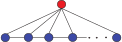
\includegraphics{fig1a}
    \caption{neighbor scaling}
    \label{fig:}
    \lfig{network_a}
  \end{center}
\end{figure}
%---end figure network a--------------------------------

We introduce a social polling sampler called \texttt{Ideal} sampler that circumvents this bias by dividing each $f(v)$ by $d_v$. The pseudo-code is shown in Alg. 2.
We are going to provide a proof that this sampler is indeed unbiased and again present bounds on the sampling size.
%---algo2----------------------------------------------
\begin{algorithm*}[!htb]
\caption{\small {\bf Ideal size sampler}($G, f, r, p$)}
\begin{code}
{\bf Input:} Graph $G=(V,E)$, function $f : V \rightarrow \{0,1\}$, sample size $r$,\\ distribution $p$ \\
{\bf Output:} $\hat{f}=\frac{1}{nr}\sum\nolimits_{u\in S}\frac{1}{p_u}\sum\nolimits_{v\in N(u)} f(v)/d_v$\\
\\
\uln \>\ubegin\\
\uln \>\>initialize $f^*$ with 0 \\
\uln \>\>randomly draw a set $S$ with r samples from $V$ with\\
\>   \>\>probability $p_u$ and with replacement\\
\uln \>\>\ufor each $u \in S$ \udo\\
\uln \>\>\>\ufor each $v \in N(u)$ \udo\\
\uln \>\>\>\>$f^* = f^* + \frac{1}{p_u}f(v)/d_v$ \\
\uln \>\>\>\uend\\
\uln \>\>\uend\\
\uln \>\ureturn $\hat{f} = \frac{f^*}{nr}$ \\
\uln \>\uend\\ 
\end{code}
\label{algideal}
\end{algorithm*}
%---end algo2------------------------------------------

First and foremost, we introduce $A$ as adjacency matrix of the graph $G$, which means $A_uv = 1$ if and only if $(u,v) \in E$. $D$ is called the diagonal matrix such that $D_{uu} = d_u$.
Let the diagonal matrix $P$ be $P_{uu} = p_u$ with $\sum\nolimits_{u}p_u$ for any vector $p \in \mathbb{R}^n$.
We also introduce $\mathds{F}$ which is the indicator (column) vector of the set ${u\;|\;f(u)=1}$, i.e., $\mathds{F}_u=f(u)$.
$\mathds{1}$ is simply an $n$-element vector of all 1's.
Our \texttt{Ideal} sampler is defined with $F = \sum_{u}\frac{e_u^TAD^{-1}\mathds{F}}{np_u}$ as $\hat{f} = F/r$.

\begin{lemma}
  The random variable $F$ satisfies $E[F] = \mathds{F}/n$ and \\
  $E[F^2] = \frac{1}{n^2}\mathds{F}^TD^{-1}AP^{-1}AD^{-1}\mathds{F}$.
\end{lemma}
\textbf{\textit{Proof: }}
\begin{align*}
\textbf{E}[F] \quad&=\quad \sum_u p_u \frac{e_u^TAD^{-1}\mathds{F}}{np_u} \quad=\quad \sum_u e_u^TAD^{-1}\mathds{F}/n \\
&=\quad\mathds{1}^TAD^{-1}\mathds{F}/n \quad=\quad DD^{-1}\mathds{F}/n \quad=\quad \mathds{F}/n \\
\textbf{E}[F^2] \quad&=\quad \sum_u p_u \bigg(\frac{e_u^TAD^{-1}\mathds{F}}{np_u}\bigg)^2 \quad=\quad \frac{1}{n^2}\sum_u \frac{(e_u^TAD^{-1}\mathds{F})^2}{p_u} \\
&=\quad\frac{1}{n^2}\sum_u \mathds{F}^TD^{-1}Ae_ue_u^TAD^{-1}\mathds{F}/p_u \\
&=\quad \mathds{F}^TD^{-1}A\bigg(\sum_ue_ue_u^T/p_u\bigg)AD^{-1}\mathds{F}/n^2 \\
&=\quad \mathds{F}^TD^{-1}AP^{-1}AD^{-1}\mathds{F}/n^2
\end{align*}
Since $\mathds{F}/n$ is a vectorial way of expressing the fraction $\bar{f}$ the estimator is indeed unbiased.

We still want to find a bound for the number of samples, similar to the \texttt{Naive} sampler.
Therefore we first provide a bound for the variance in the special case where nodes $u$ are sampled with probability proportional $|N(u)| = d_u$.

\begin{lemma}
  Let the sampling probability be $p_u = \frac{d_u}{2m}$. Then $\textbf{var}(F) \leq (2m/n^2)\lambda_2^2||D^{-1/2}f||^2$ with $\lambda_2$ being the second largest eigenvalue of matrix $L = D^{-1/2}AD^{-1/2}$. 
\end{lemma}
\textbf{\textit{Proof: }}
\begin{align*}
\textbf{var}(F) \quad&=\quad \textbf{E}[F^2] - (\textbf{E}[F])^2 \quad=\quad \mathds{F}^TD^{-1}AP^{-1}AD^{-1}\mathds{F}/n^2 - (\mathds{F}/n)^2 \\
&=\quad \mathds{F}^TD^{-1}A(2mD^{-1})AD^{-1}\mathds{F}/n^2 - (\mathds{F}/n)^2\\
&=\quad \frac{2m}{n^2}\mathds{F}^TD^{-1}AD^{-1}AD^{-1}\mathds{F} - (\mathds{F}/n)^2\\
&=\quad \frac{2m}{n^2}\mathds{F}^TD^{-1/2}L^2D^{-1/2}\mathds{F}-\mathds{F}^T\mathds{1}\mathds{1}^T\mathds{F}/n^2\\
&=\quad \frac{2m}{n^2}\mathds{F}^TD^{-1/2}\bigg(L^2-\frac{D^{1/2}\mathds{1}\mathds{1}^TD^{1/2}}{2m}\bigg)D^{-1/2}\mathds{F}\\
&\leq\quad \frac{2m}{n^2}\bigg|\bigg|L^2 - \frac{D^{1/2}\mathds{1}\mathds{1}^TD^{1/2}}{2m}\bigg|\bigg|||D^{-1/2}\mathds{F}||^2
\end{align*}
One can show by using linear algebra that $\lambda_2^2 = ||L^2 - \frac{D^{1/2}\mathds{1}\mathds{1}^TD^{1/2}}{2m}||$.

We can now use this bound and the Chebyshev inequality to prove the following bound on $r$.

\begin{theorem}
Using $r = \frac{2\textbf{var}(F)}{\epsilon^2\delta}$ and $p_u = \frac{d_u}{2m}$, with probability $1-\delta$ the \texttt{Ideal} sampler will give an estimate $\hat{f}$ such that $|\hat{f}-\bar{f}|< \epsilon$.  
\end{theorem}
\textbf{\textit{Proof: }}
\begin{align*}
\textbf{Pr}[|\hat{f}-\bar{f}|\;>\epsilon] \quad&\leq\quad \frac{2\textbf{var}(\hat{f})}{\epsilon^2} \quad\leq\quad \frac{2\textbf{var}(\hat{F})}{r\epsilon^2} \\
&\leq\quad \frac{2\textbf{var}(F)\epsilon^2\delta}{2\textbf{var}(F)\epsilon^2} \quad\leq\quad \delta
\end{align*}

\subsection{\texttt{Sparse} sampler}
The \texttt{Ideal} sampler samples all neighbors of the sampled node. Thinking back to social network this means a person is expected to represent all of their neighbors choices.
Now, we present a variant of this estimator that only samples a subset $T_u$ of $u$'s neighbors.
This represents a scenario where either polling all neighbors is expensive respectively impossible (e.g. API limitations) or where we use further heuristics to select an arbitrary amount of neighbors. In the second case one could think of a poll like "\textit{Think of three of your female friends and tell us how many are married.}".

Be aware that this sampler uses an additional parameter called $k$. This is the size of set $T'_u$, a randomly chosen subset from $T_u$.
We are aware this contradicts the initial definition of a sampler but we since $k$ has no usage in the other samplers we will stick to this defintition.

In this implementation we will pick each neighbor with probability inversly proportional to their degrees and pick the subset of $k$ neighbors with probability $1/|T_u|$.

There are no proofs on the bound of the sample size yet and deriving one is considered out of the scope of this paper.
%---algo3----------------------------------------------
\begin{algorithm*}[!htb]
\caption{\small {\bf Sparse size sampler}($G, f, r, p, k$)}
\begin{code}
{\bf Input:} Graph $G=(V,E)$, function $f : V \rightarrow \{0,1\}$, sample size $r$,\\ distribution $p$, parameter $k$ \\
{\bf Output:} $\hat{f}=\frac{1}{nr}\sum\nolimits_{u\in S}\frac{1}{p_u}(|T_u|/k)\sum\nolimits_{v\in T'_u} f(v)$\\
\\
\uln \>\ubegin\\
\uln \>\>initialize $f^*$ with 0 \\
\uln \>\>randomly draw a set $S$ with r samples from $V$ with\\
\>   \>\>probability $p_u$ and with replacement\\
\uln \>\>\ufor each $u \in S$ \udo\\
\uln \>\>\>1. randomly draw a set $T_u$ by picking each neighbor\\
\>   \>\>\> $v \in N(u)$ with probability $1/d_v$ \\
\uln \>\>\>2. randomly draw a set $T'_u \subseteq T_u$ by picking\\
\>   \>\>\> $k$ elements of $T_u$ without replacement with\\
\>   \>\>\> probability $1/|T_u|$.\\
\uln \>\>\>\ufor each $v \in T'_u$ \udo\\
\uln \>\>\>\>$f^* = f^* + \frac{1}{p_u}(|T_u|/k)f(v)$ \\
\uln \>\>\>\uend\\
\uln \>\>\uend\\
\uln \>\ureturn $\hat{f} = \frac{f^*}{nr}$ \\
\uln \>\uend\\ 
\end{code}
\label{algsparse}
\end{algorithm*}
%---end algo3------------------------------------------
\subsection{\texttt{Expectation} sampler}
The final presented sampler is based on the research of Rothschild and Wolfers in \cite{rothschild2009forecasting}. They showed with statistical measurements that using a method called "expectation polling" can lead to significantly better estimations than the classical "intent polling".
In practise this means posing a "\textit{Which party will win the next vote?}" instead of "\textit{Who do you vote for?}".
They base this on the assumption that a respondent often gives an aggregate view of its friends and family (i.e. neighbors in a social network).
The presented algorithm that aims to implement expectation polling let each sampled node $u$ report a fraction instead of a simple 0/1. The fraction represents the estimatated fraction of the neighbors with $f(v) = 1$.
Compared with the \texttt{Ideal} sampler there exist a similar bound on $r$ and we present this without a proof:
\begin{theorem}
Using $r = \frac{4m\lambda_2^2||D^{-1/2}\mathds{F}||||D^{-1/2}(\mathds{1}-\mathds{F})||}{n^2\epsilon^2\delta}$, with probability $1-\delta$ the \texttt{Expectation} sampler will give an estimate $\hat{f}$ such that $|\hat{f}-\bar{f}|< \epsilon$.  
\end{theorem}
%---algo4----------------------------------------------
\begin{algorithm*}[!htb]
\caption{\small {\bf Expec winner sampler}($G, f, r, p$)}
\begin{code}
{\bf Input:} Graph $G=(V,E)$, function $f : V \rightarrow \{0,1\}$, sample size $r$,\\ distribution $p$ \\
{\bf Output:} $\hat{f}=\frac{1}{nr}\sum\nolimits_{u\in S}\frac{1}{p_u}G(u)$\\
\\
\uln \>\ubegin\\
\uln \>\>initialize $f^*$ with 0 \\
\uln \>\>randomly draw a set $S$ with r samples from $V$ with\\
\>   \>\>probability $p_u$ and with replacement\\
\uln \>\>\ufor each $u \in S$ \udo\\
\uln \>\>\>1. compute $q_u = \sum_{v\in N_u}\frac{f_v}{d_v}$\\
\>   \>\>\>2. compute $r_u = \sum_{v\in N_u}\frac{1}{d_v}$\\
\>   \>\>\>3. flip coin with probability $\frac{q_u}{r_u}$\\
\uln \>\>\>\uif heads\\
\uln \>\>\>\>$f^* = f^* + r_u$ \\
\uln \>\>\>\uelse\\
\uln \>\>\>\>$f^* = f^* + 0$ \\
\uln \>\>\>\uend\\
\uln \>\>\uend\\
\uln \>\ureturn $\hat{f} = \frac{f^*}{nr}$ \\
\uln \>\uend\\ 
\end{code}
\label{algexpec}
\end{algorithm*}
%---end algo4------------------------------------------


\section{Results}
Dasgupta et al. \cite{dasgupta2012social} performed various experiments to measure the performance of the samplers.
They focused on two large, publically available databases.

The \texttt{LiveJournal} network contains 5.36M nodes and approximately 160M edges and is based on a snapshot of the social network livejournal.com in March 2008.
The \texttt{DBLP} network contains 368K nodes and 8M edges and consists of the content of the DBLP database located on http://www.informatik.uni-trier.de/~ley/db/.


\bibliographystyle{abbrv}
\bibliography{bibliography}

\end{document}
